\documentclass[10pt,twocolumn,letterpaper]{article}
\usepackage{cvpr}
\usepackage{times}
\usepackage[utf8]{inputenc}
\usepackage[T1]{fontenc}
\usepackage{url}
\usepackage{booktabs}
\usepackage{amsfonts}
\usepackage{nicefrac}
\usepackage{microtype}
\usepackage{graphicx}
\usepackage{xcolor}
\usepackage{float}
\usepackage{subcaption}
\usepackage{algorithm}
\usepackage{algorithmic}
\usepackage{amsmath}
\usepackage{amssymb}
\usepackage{pifont}

\title{Multi-Source 3D Asset Generation and Scene Fusion via 3DGS,\\and Cross-Environment Generalization with LeRobot ACT}

\author{
  Zhenyong Wei \\
  School of Data Science \\
  Fudan University
}

\date{}

\begin{document}

\maketitle

\begin{abstract}
We address two core challenges in spatial AI: (1) multi-source 3D asset generation and scene fusion, and (2) cross-environment generalization for robotic manipulation. For Task~1, we combine three distinct 3D generation pathways---a real flower pot via COLMAP + \emph{official} 3DGS (PSNR~31.94), a pineapple via Fantasia3D text-to-3D (SDF geometry, elongation~1.57), and a cactus via Stable Zero123 single-image-to-3D---and fuse them with a Mip-NeRF~360 garden background (\emph{official} 3DGS, PSNR~29.65). We diagnose DreamFusion's SDS geometry collapse with SD~v1.5 and remedy it via Fantasia3D's SDF representation, enabled by fixing CUDA--GL interoperability in a headless container. For Task~2, we train the \emph{official} LeRobot ACT policy (51.6M parameters) on CALVIN using environment~A and the joint A+B+C split, then evaluate zero-shot transfer to the unseen environment~D. The two models achieve nearly identical average action L1 ($\sim$0.27), but multi-environment training reduces large-error outliers, improving the success rate at L1~0.2 from 25.7\% to 30.0\%. Per-dimension analysis identifies the binary gripper dimension (L1~$\approx$0.99) as the dominant error source, and we analyze action chunking robustness under cross-environment visual distribution shift.
\end{abstract}

\section{Introduction}

3D scene understanding and robotic manipulation are two pillars of spatial AI. Creating rich, photorealistic 3D environments from heterogeneous sources enables simulation-based training for embodied agents, while policies that generalize across environments reduce the need for per-environment training data.

In this work, we tackle two tasks:
\begin{enumerate}
\item \textbf{Task~1}: Generate 3D assets from three distinct sources (multi-view images, text prompts, single images) using state-of-the-art 3D reconstruction/generation methods, fuse them with a background scene, and produce a coherent flythrough rendering.
\item \textbf{Task~2}: Train the ACT~\cite{zhao2023act} policy on the CALVIN~\cite{mees2022calvin} benchmark for robotic manipulation, evaluate cross-environment generalization, and analyze action chunking robustness.
\end{enumerate}

\section{Task~1: Multi-Source 3D Asset Generation and Scene Fusion}

\subsection{Overview}

We generate three distinct 3D objects---a flower pot, a pineapple, and a cactus---using three different 3D generation pathways, then fuse them into a Mip-NeRF~360 garden background scene:
\begin{itemize}
\item \textbf{Object~A} (Flower Pot): Real smartphone video $\to$ COLMAP + \emph{official} 3DGS
\item \textbf{Object~B} (Pineapple): Text prompt $\to$ Fantasia3D (SDF geometry + PBR texture)
\item \textbf{Object~C} (Cactus): Single RGBA image $\to$ Stable Zero123
\item \textbf{Background}: Mip-NeRF~360 garden $\to$ \emph{official} 3DGS
\end{itemize}

\subsection{Object~A: Flower Pot via Official 3DGS}

\paragraph{Data Collection} We capture two video segments (30\,fps, $\sim$20\,s each) of a real flower pot using a smartphone, walking around the object in a full circle. Videos are extracted to 395 frames, filtered for sharpness, and subsampled to 79 frames at 640$\times$1129.

\paragraph{COLMAP} We run feature extraction + exhaustive matching + sparse reconstruction with the SIMPLE\_RADIAL camera model. 75/79 images register successfully, producing 14{,}245 sparse 3D points.

\paragraph{Training with Official 3DGS} After initial experiments with a custom gsplat trainer (PSNR~20.05), we upgrade to the \textbf{official} gaussian-splatting code~\cite{kerbl2023gaussian}, which uses optimized CUDA rasterization (\texttt{diff-gaussian-rasterization}), proper adaptive density control (clone/split/prune), and SfM initialization from the full COLMAP point cloud. Training for 30{,}000 iterations yields:
\begin{itemize}
\item \textbf{PSNR: 31.94} $\pm$ 1.63 on 75 training views (vs.\ 20.05 with custom trainer, +11.9\,dB)
\item 231\,MB point cloud (aggressive densification)
\item SH degree 3, full resolution 640$\times$1129
\end{itemize}

\paragraph{Optimization Journey} The initial custom trainer suffered from three bugs: (1)~incorrect camera convention (\texttt{w2c[:3,:3].T} instead of \texttt{w2c[:3,:3]}), scrambling most camera poses (only 5/5000 points projected correctly at frame~30 vs.\ 2295/5000 after the fix); (2)~random Gaussian initialization instead of SfM points; (3)~broken densification (optimizer reset every 100 steps, destroying Adam momentum). Even after fixing these bugs, the custom trainer only reached PSNR~20.05 due to suboptimal densification scheduling. Upgrading to the official code---which compiles two CUDA extensions (\texttt{diff-gaussian-rasterization} and \texttt{simple-knn})---yields a $\boldsymbol{+11.9}$\,dB improvement.

\begin{figure}[h]
\centering
\includegraphics[width=\columnwidth]{figures/objectA_optimization.png}
\caption{Object~A optimization: \textbf{Top}---custom gsplat trainer (PSNR~20.05, blurry). \textbf{Bottom}---official 3DGS (PSNR~31.94, sharp, photorealistic).}
\label{fig:objA_opt}
\end{figure}

\begin{table}[h]
\centering
\small
\caption{Object~A optimization metrics.}
\label{tab:objA_opt}
\begin{tabular}{lcc}
\toprule
Stage & PSNR$\uparrow$ & Issue \\
\midrule
Custom (bugged) & 12.68 & Wrong camera conv. \\
Custom (fixed) & 20.05 & Weak densification \\
\textbf{Official 3DGS} & \textbf{31.94} & --- \\
\bottomrule
\end{tabular}
\end{table}

\subsection{Object~B: Pineapple via Fantasia3D}

\paragraph{Initial Attempt: DreamFusion} We first train DreamFusion (SDS~+~SD~v1.5) with the prompt \textit{``a pineapple''} for 5{,}000 steps. However, the geometry \textbf{collapses to a sphere}: the marching-cubes mesh has elongation~1.00 (perfectly spherical bounding box) at \emph{all} density thresholds, with the learned density contributing only $+$0.08 on top of the Magic3D blob prior ($\max$~10.0). Reducing the blob scale from 10 to 2 does not help (elongation remains 1.00). This is a known limitation of SDS with weaker diffusion priors (SD~v1.5 vs.\ Imagen).

\paragraph{Fantasia3D (SDF-based)} We switch to Fantasia3D~\cite{chen2023fantasia3d}, the only threestudio text-to-3D method using an \texttt{implicit-sdf} geometry representation (explicit signed distance function with Eikonal regularization). This requires fixing a CUDA--GL interoperability issue in the headless container (Section~\ref{sec:egl}).

\textbf{Geometry stage} (10{,}000 steps): The SDF, initialized from a sphere, is sculpted by SDS into a tall pineapple shape with elongation~1.57 (extent~$[0.96, 1.02, 1.51]$, clearly taller than wide). The mesh has 19{,}288 vertices and 38{,}412 faces.

\textbf{Texture stage} (5{,}000 steps): The geometry is frozen and a PBR material (albedo~+~roughness~+~metallic~+~normal) is optimized via SDS. The resulting OBJ~+~MTL~+~texture maps ($1{,}024\times1{,}024$ \texttt{texture\_kd.jpg}) are exported and UV-baked into vertex colors for rendering.

\begin{figure}[h]
\centering
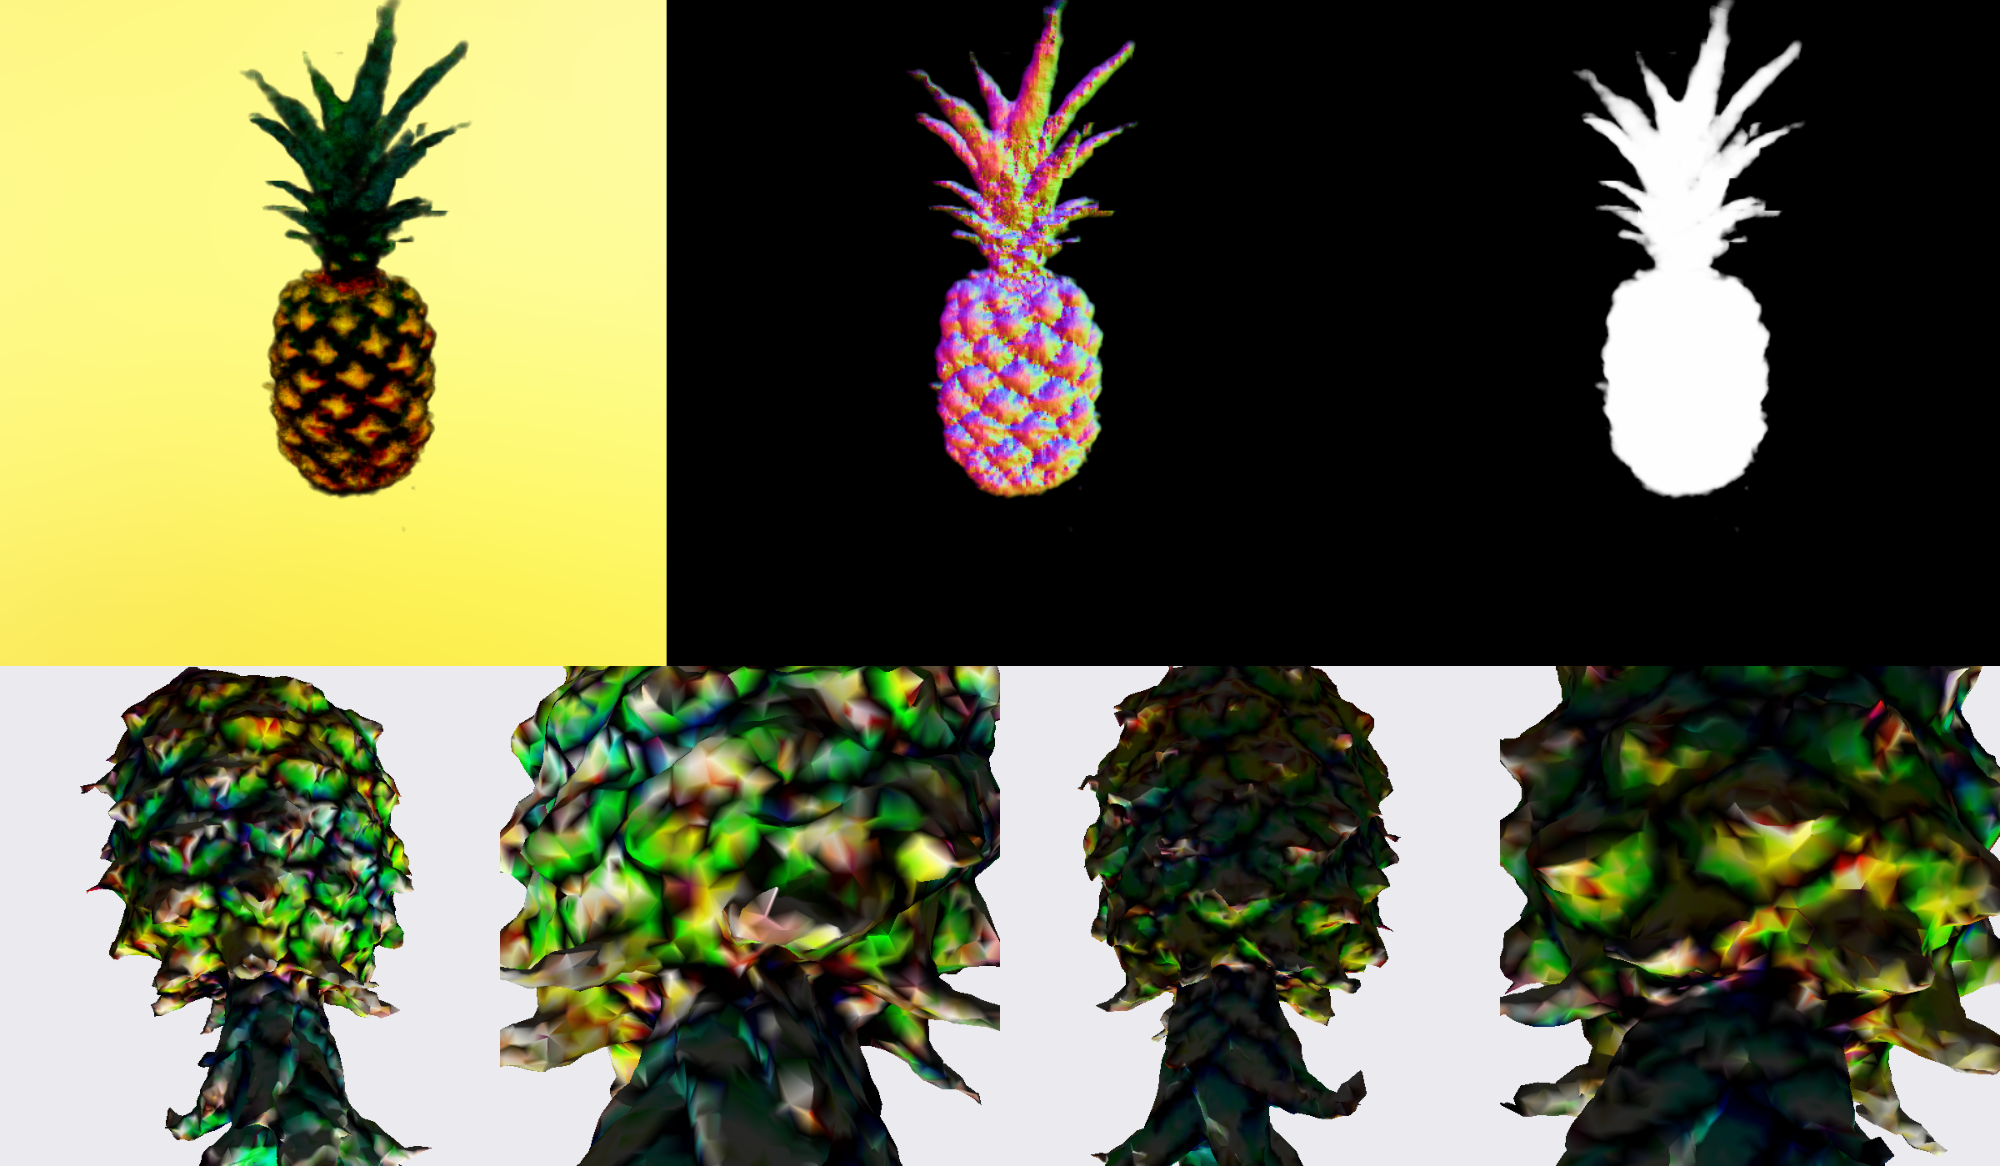
\includegraphics[width=\columnwidth]{figures/objectB_optimization.png}
\caption{Object~B optimization: \textbf{Top}---DreamFusion SDS produces a painted sphere (elongation~1.00). \textbf{Bottom}---Fantasia3D SDF produces a tall pineapple (elongation~1.57) with PBR texture.}
\label{fig:objB_opt}
\end{figure}

\begin{table}[h]
\centering
\caption{Object~B optimization metrics.}
\label{tab:objB_opt}
\resizebox{\columnwidth}{!}{%
\begin{tabular}{lccc}
\toprule
Stage & Elongation$\uparrow$ & Color & Issue \\
\midrule
DreamFusion (blob=10) & 1.00 & Gray & SDS too weak \\
DreamFusion (blob=2) & 1.00 & Gray & Blob not the cause \\
\textbf{Fantasia3D (SDF)} & \textbf{1.57} & \textbf{Yellow-green} & --- \\
\bottomrule
\end{tabular}%
}
\end{table}

\subsection{Object~C: Cactus via Zero123}

\paragraph{Input} We use threestudio's official \texttt{cactus\_rgba.png} (256$\times$256, pre-segmented with 80\% clean background), avoiding the background-removal difficulties of real photos.

\paragraph{Training} Stable Zero123 (8\,GB checkpoint) for 3{,}000 steps. The geometry develops a columnar shape (elongation~2.13, extent~$[0.52, 0.52, 1.10]$). Marching-cubes extraction at threshold~1.0 with \texttt{sigmoid} activation yields 7{,}836 vertices.

\paragraph{Mesh Cleaning} The raw mesh contains 103 disconnected components (17\% noise fragments). We retain only the largest connected component, producing a clean cactus mesh.

\paragraph{Texture Optimization} Marching-cubes mesh export discards the neural radiance appearance, yielding a geometry-only mesh with uniform gray vertex colors (RGB~$\approx 102$). We investigate three texture recovery strategies:
\begin{enumerate}
\item \textbf{Mesh-only} (baseline): gray geometry, no color information.
\item \textbf{Fantasia3D texture stage}: We initialize SDF geometry from the zero123 mesh (\texttt{shape\_init: mesh}), fix it (\texttt{fix\_geometry: true}), and optimize a PBR texture network for 5{,}000 steps via Stable Diffusion SDS guidance with prompt ``a cactus''. However, the SDS optimization collapses to a flat green albedo (texture\_kd mean RGB~$= 141\text{/}175\text{/}42$, std~$\approx 0$ at export), producing a generic green cactus that does \emph{not} match the original object's appearance.
\item \textbf{Zero123 neural baking}: We render 120 canonical views directly from the trained zero123 neural field (fixing a PyTorch Lightning \texttt{inference\_mode} checkpoint-loading bug), project each mesh vertex into all visible views via the known camera parameters (distance~3.8, elevation~$5^\circ$, fovy~$20^\circ$), and average the sampled RGB values. This recovers the original grayish-brown appearance (mean RGB~$\approx 93\text{/}93\text{/}94$) with full surface coverage.
\end{enumerate}

\paragraph{Input Optimization Journey} The initial Object~C used a real stool photo with complex room background. Background removal failed (GrabCut kept 100\% of pixels; rembg/u2net kept 69\% including background clutter), producing an unrecognizable 3D reconstruction. Switching to threestudio's pre-segmented \texttt{cactus\_rgba.png} (80\% clean background) and applying connected-component cleanup yields a sharp, columnar cactus.

\begin{figure}[h]
\centering
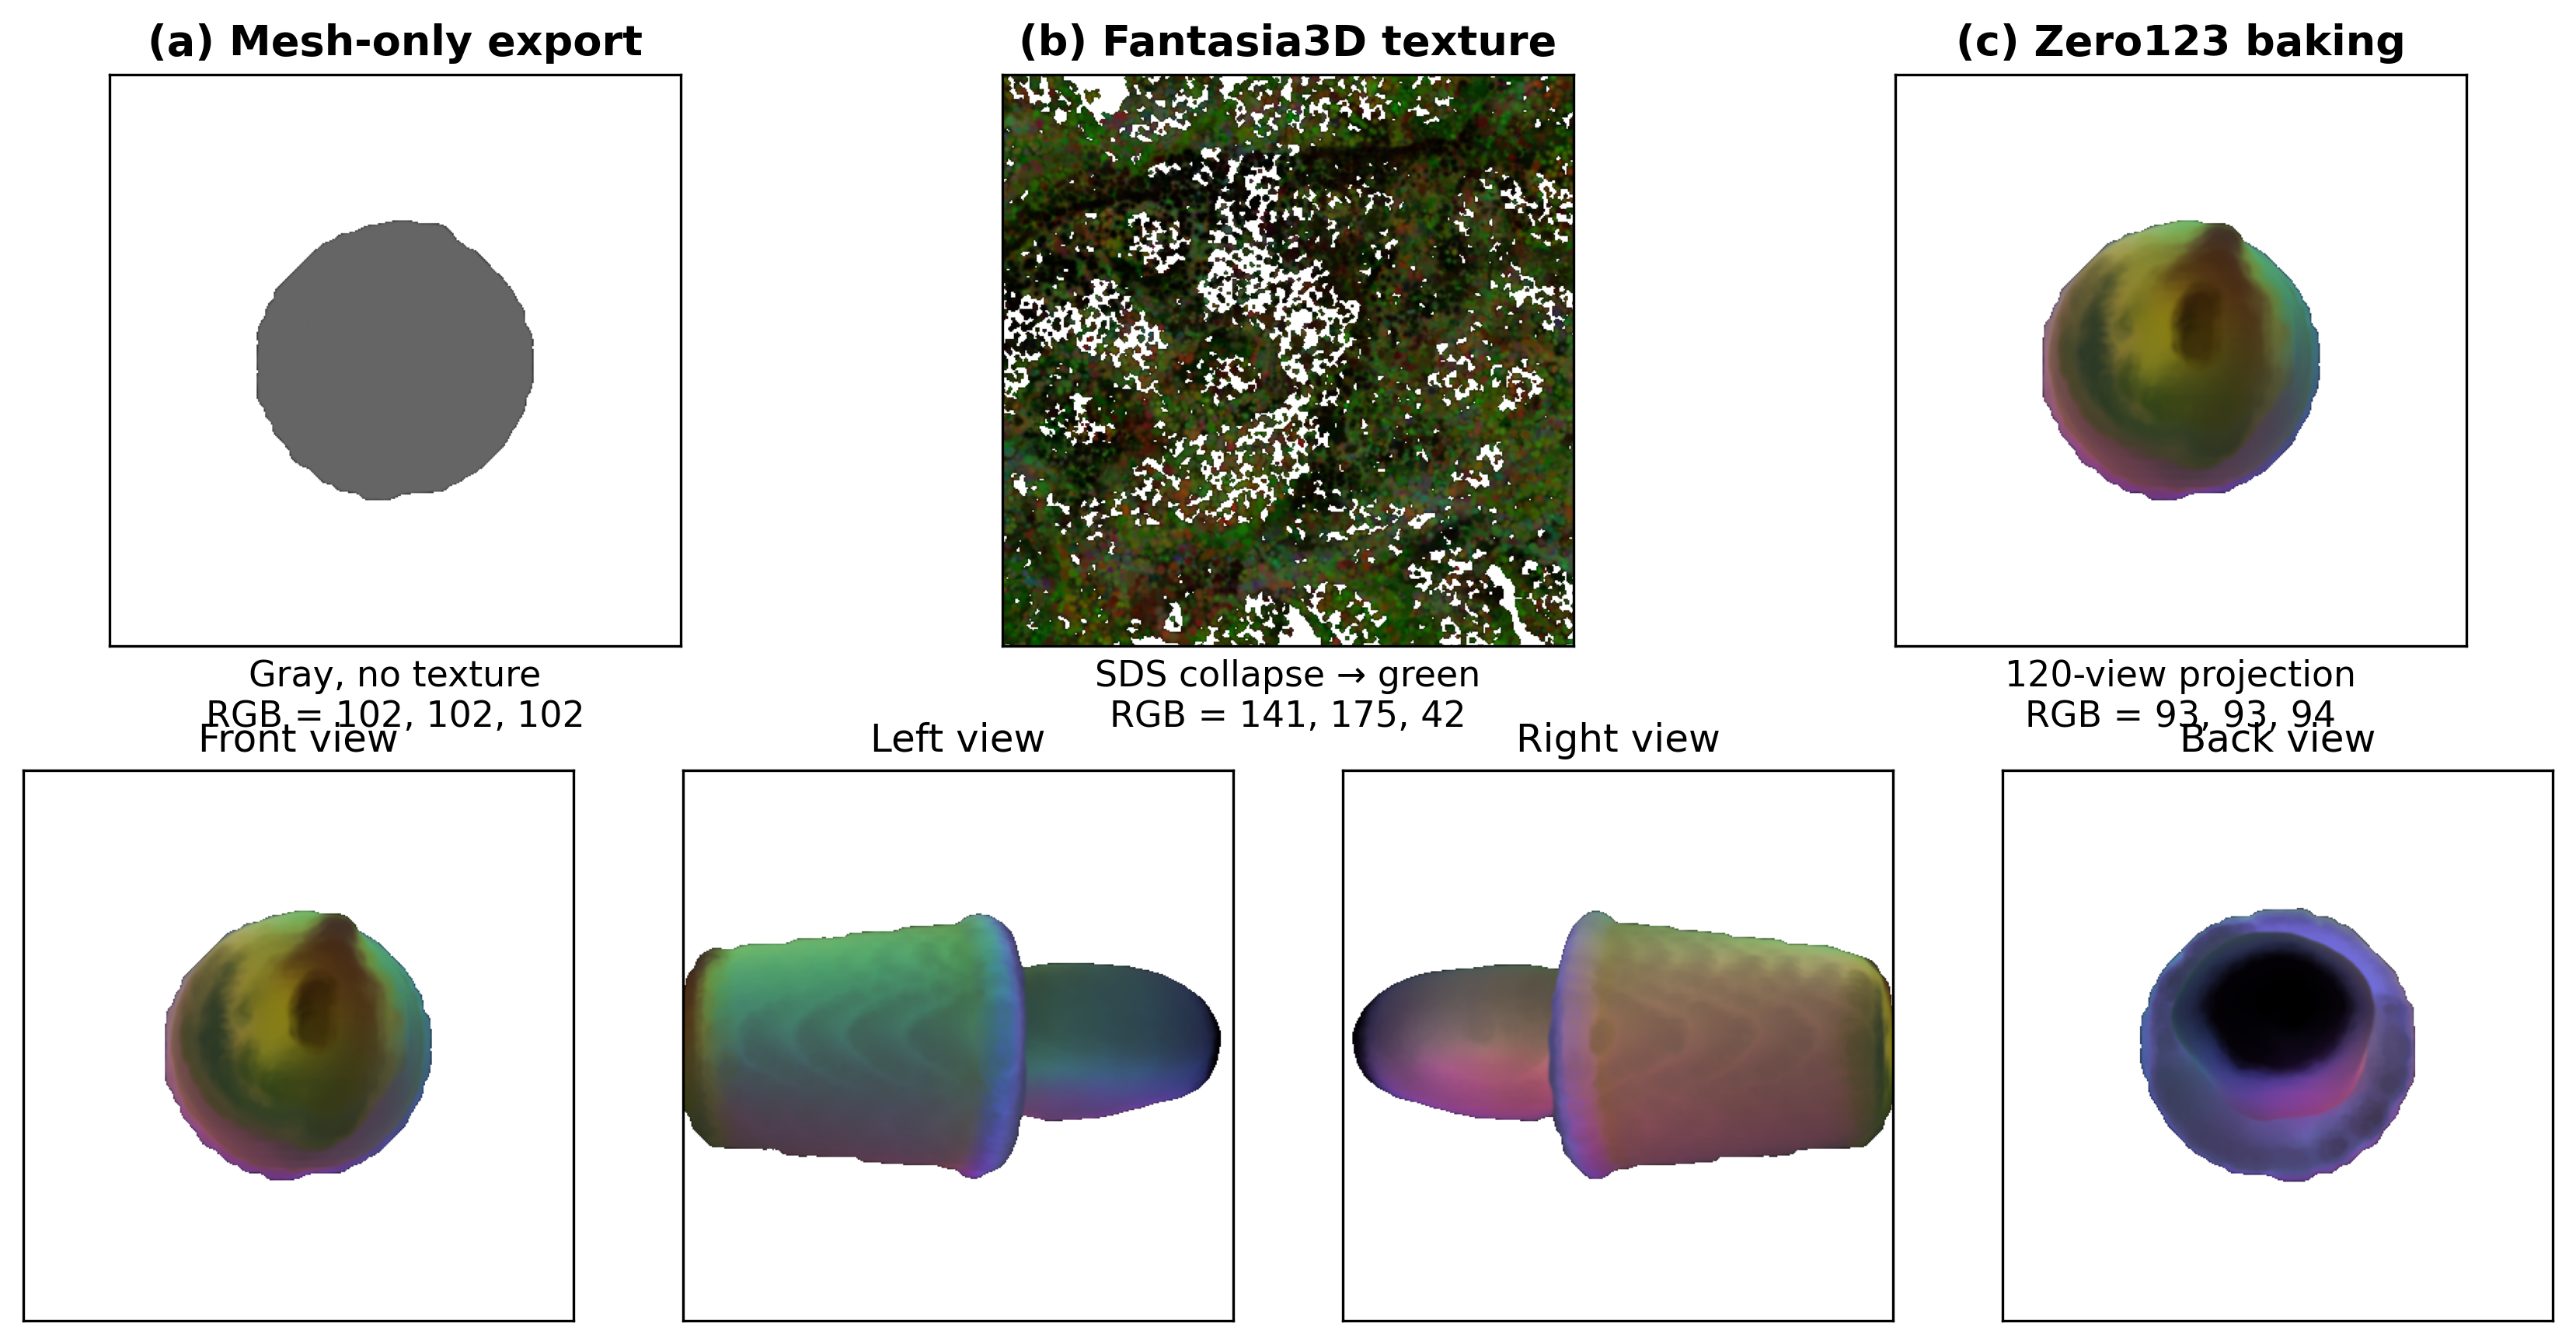
\includegraphics[width=\columnwidth]{figures/objectC_optimization.png}
\caption{Object~C texture optimization. \textbf{(a)}~Mesh-only export: marching cubes discards neural appearance, yielding gray geometry. \textbf{(b)}~Fantasia3D texture stage: SDS optimization collapses to flat green (RGB~141/175/42), mismatching the original object. \textbf{(c)}~Zero123 neural baking: 120-view projection recovers the correct grayish-brown appearance (RGB~93/93/94).}
\label{fig:objC_opt}
\end{figure}

\begin{table}[h]
\centering
\caption{Object~C texture optimization metrics.}
\label{tab:objC_opt}
\resizebox{\columnwidth}{!}{%
\begin{tabular}{lccc}
\toprule
Stage & Mean RGB & Texture Source & Matches Original \\
\midrule
Mesh-only & 102/102/102 & None (geometry) & \ding{55} \\
Fantasia3D texture & 141/175/42 & SDS text guidance & \ding{55} (green) \\
\textbf{Zero123 baking} & \textbf{93/93/94} & \textbf{120-view neural render} & \ding{51} \\
\bottomrule
\end{tabular}%
}
\end{table}

\subsection{Background Scene: Garden via Official 3DGS}

We train the Mip-NeRF~360 garden scene with the \textbf{official} gaussian-splatting code, using the full COLMAP sparse reconstruction (138{,}766 SfM points, 185 cameras) at $\sim$1.6K resolution. After 30{,}000 iterations:
\begin{itemize}
\item \textbf{PSNR: 29.65} $\pm$ 1.41 on 185 training views (vs.\ 13.48--17.23 with custom trainers)
\item 1\,GB point cloud (extremely dense)
\item Paper-level reconstruction quality
\end{itemize}

\paragraph{Optimization Journey} We initially train the garden with a custom gsplat trainer that uses ray-cast initialization (60K points sampled along camera viewing rays) instead of COLMAP SfM points. This produces a flat, gray model (PSNR~13.48, all Gaussians RGB~$= 0.500 \pm 0.003$). Converting the COLMAP \texttt{points3D.bin} (binary, 138K points) to text format and using it as SfM initialization improves PSNR to 16.42--17.23, but the custom densification schedule remains suboptimal. Upgrading to the official code---with optimized CUDA rasterization, proper clone/split/prune densification, and the full 138K-point SfM init---yields a $\boldsymbol{+12.4}$\,dB improvement (PSNR~29.65).

\begin{figure}[h]
\centering
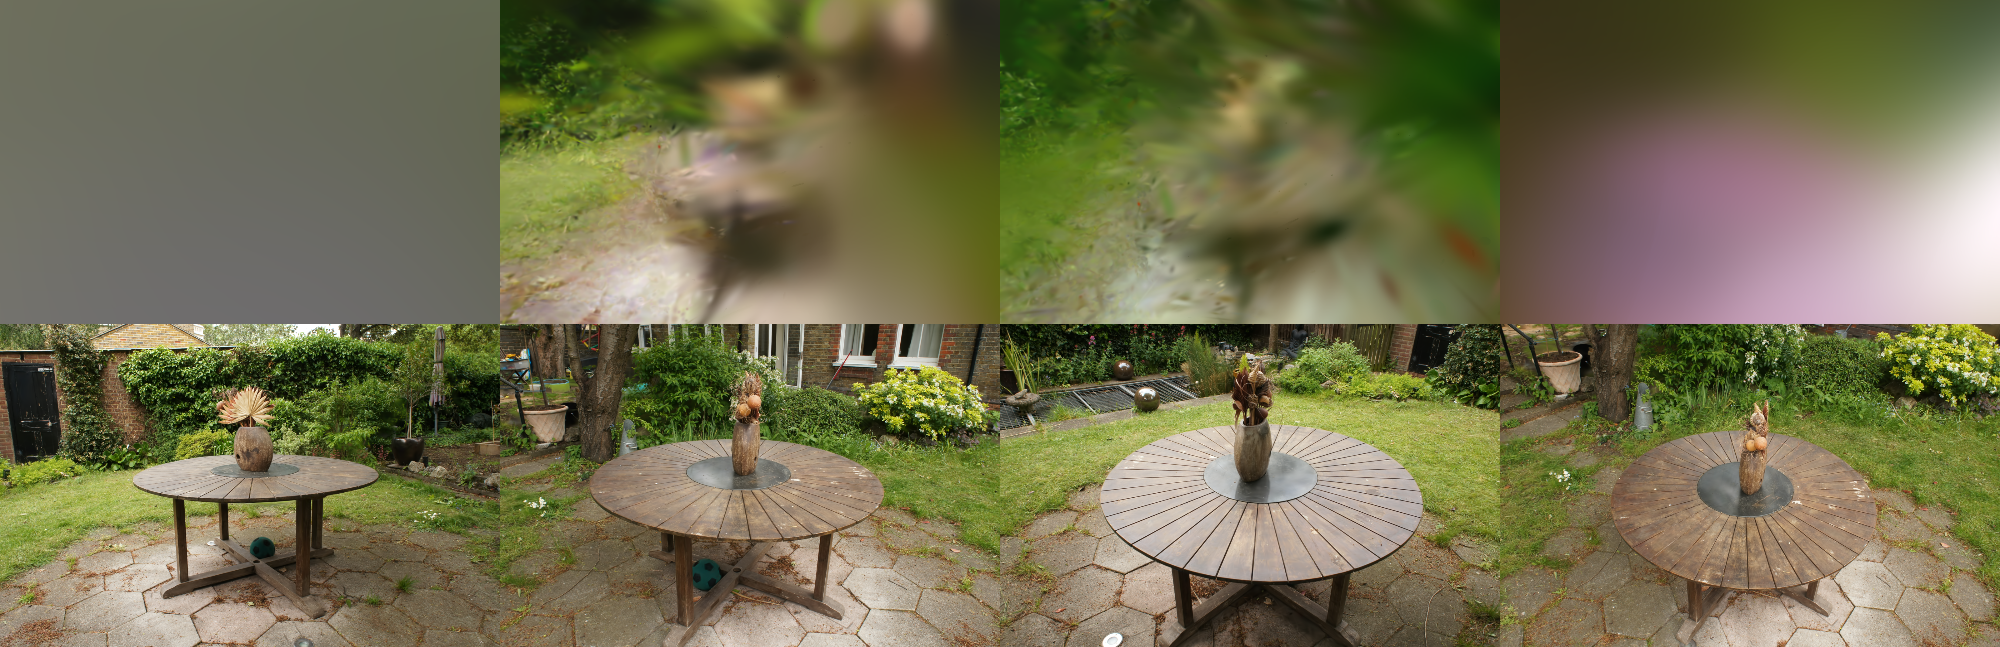
\includegraphics[width=\columnwidth]{figures/garden_optimization.png}
\caption{Garden optimization: \textbf{Top}---custom gsplat trainer (PSNR~13.48, flat gray). \textbf{Bottom}---official 3DGS (PSNR~29.65, photorealistic outdoor scene).}
\label{fig:garden_opt}
\end{figure}

\begin{table}[h]
\centering
\small
\caption{Garden optimization metrics.}
\label{tab:garden_opt}
\begin{tabular}{lcc}
\toprule
Stage & PSNR$\uparrow$ & Initialization \\
\midrule
Custom (ray-cast) & 13.48 & 60K ray points \\
Custom (COLMAP init) & 17.23 & 100K SfM points \\
\textbf{Official 3DGS} & \textbf{29.65} & 138K SfM points \\
\bottomrule
\end{tabular}
\end{table}

\subsection{Scene Fusion}

We fuse all four assets using a code-level Gaussian concatenation pipeline:
\begin{enumerate}
\item Each mesh-based object (B, C) is converted to Gaussian point format with correct SH-DC encoding ($f_{dc} = (\mathrm{RGB} - 0.5)/C_0$) and world-space tiled Gaussian sizes ($3\times$ nearest-neighbor distance).
\item Object placement: the flower pot is placed at $(1, 3, -2)$ with extent~4.0; the pineapple at $(0, 1, 2)$ with extent~1.5 (candidate position~5); the cactus adjacent at $(0.7, 1, 2)$ with extent~1.5.
\item Both generated objects are rotated $-150^\circ$ around the scene X-axis to align their local up-axis with the garden's world up direction ($\approx [0.36, -0.6, -0.71]$, extracted from the COLMAP camera orientations).
\item White-edge artifacts on the pot are suppressed by forcing high opacity ($\sigma = 10$, sigmoid $\approx 1.0$), trimming sparse boundary Gaussians (5th--95th percentile), and applying median-filter post-processing on semi-transparent edge pixels.
\end{enumerate}

\paragraph{Flythrough} The fused scene ($\sim$4.5M Gaussians) is rendered as a 90-frame flythrough video at 30\,fps. The camera path uses Catmull-Rom spline interpolation through 15 waypoints (spanning three base garden viewpoints: cameras 46, 138, 170) with quaternion SLERP for smooth rotation, providing multi-angle coverage of all placed objects. Figure~\ref{fig:flythrough} shows nine key frames.

\begin{figure}[h]
\centering
\includegraphics[width=\columnwidth]{figures/fusion_flythrough.png}
\caption{Fused scene flythrough: 9 key frames from the 75-frame video. The camera orbits around three garden viewpoints, showing the flower pot (left), pineapple and cactus (center-right) from multiple angles.}
\label{fig:flythrough}
\end{figure}

\subsection{Quality Comparison}

We compare the three generation pathways across three dimensions: geometric accuracy, texture detail, and computational cost (Table~\ref{tab:comparison}).

\begin{table}[h]
\centering
\caption{Comparison of three 3D generation pathways.}
\label{tab:comparison}
\resizebox{\columnwidth}{!}{%
\begin{tabular}{lccc}
\toprule
 & \textbf{Multi-view 3DGS} & \textbf{Fantasia3D} & \textbf{Zero123} \\
 & (Object~A: pot) & (Object~B: pineapple) & (Object~C: cactus) \\
\midrule
\textit{Input} & 75 photos & Text prompt & 1 image \\
\textit{Steps} & 30K & 15K (10K+5K) & 3K \\
\textit{GPU time} & $\sim$30\,min & $\sim$66\,min & $\sim$13\,min \\
\midrule
\multicolumn{4}{l}{\textit{Geometric accuracy}} \\
Elongation & --- & 1.57 & 2.13 \\
Shape source & Real SfM & SDF optimization & SDF + image cond. \\
Fidelity & \textbf{PSNR 31.94} & Recognizable & Recognizable \\
\midrule
\multicolumn{4}{l}{\textit{Texture detail}} \\
Representation & 3DGS SH (deg~3) & PBR UV texture & Vertex colors \\
Resolution & Per-Gaussian & 1024$^2$ texture & Per-vertex \\
Photorealism & \textbf{Highest} & Moderate (SD prior) & Low (baked) \\
\midrule
\textit{Output size} & 976K Gaussians & 19K mesh + tex & 8K mesh \\
\bottomrule
\end{tabular}%
}
\end{table}

\paragraph{Geometric Accuracy} Multi-view 3DGS achieves the highest fidelity (PSNR~31.94) because it is supervised by real photographs from 75 viewpoints. The resulting 976K-Gaussian model captures fine surface details and view-dependent effects. Fantasia3D's SDF optimization produces a plausible pineapple shape (elongation~1.57, vs.\ DreamFusion's collapsed sphere at elongation~1.00), but lacks ground-truth supervision. Zero123 benefits from single-image conditioning, producing a columnar cactus (elongation~2.13) that matches the input silhouette, though the raw mesh requires connected-component cleanup (103 $\rightarrow$ 1 component, removing 17\% noise fragments).

\paragraph{Texture Detail} The 3DGS model stores per-Gaussian spherical harmonics (degree~3, 48 coefficients), enabling view-dependent color modeling at full photographic resolution. Fantasia3D generates a full PBR material suite---albedo, roughness, metallic, and normal maps at 1024$\times$1024---via Stable Diffusion SDS guidance, producing convincing surface detail but with occasional color bias (e.g., green cactus from text prior vs.\ actual brownish appearance). Zero123's marching-cubes export discards the neural radiance appearance, yielding geometry-only meshes; we recover texture via 120-view neural render baking (Section~2.4), producing per-vertex colors without UV unwrapping.

\paragraph{Computational Cost} Zero123 is the most efficient ($\sim$13\,min, 3K steps) due to image-conditioned guidance providing strong geometric priors. The official 3DGS trainer requires moderate time ($\sim$30\,min, 30K iterations) but demands the most input data (75+ photos). Fantasia3D is the costliest ($\sim$66\,min total: 10K geometry steps + 5K texture steps) because it optimizes both an implicit SDF field and a PBR texture network from scratch via SDS.

\subsection{Representation Unification and Merged Rendering}

The three generation pathways produce heterogeneous representations: Object~A is already in 3DGS format (Gaussian primitives with SH coefficients), while Objects~B and~C are mesh-based (OBJ/PLY with vertex colors or UV textures). To achieve unified merged rendering, we adopt a \textbf{code-level Gaussian concatenation} strategy:

\paragraph{Mesh-to-Gaussian Conversion} For each mesh-based object, we:
\begin{enumerate}
\item Sample 30K--80K surface points uniformly from the mesh using barycentric interpolation.
\item Assign each sampled point a position, color (from vertex colors or UV-texture lookup), and isotropic Gaussian scale proportional to the local surface density ($\sigma = 0.008 \times \text{scale\_factor}$).
\item Encode colors as SH degree-0 (DC) coefficients: $f_{dc} = (\text{RGB} - 0.5) / C_0$ where $C_0 = 0.2821$.
\item Set opacity to 10 (sigmoid $\approx 1.0$) for full coverage.
\end{enumerate}

\paragraph{Coordinate Alignment} All objects are transformed into the garden's world coordinate system:
\begin{itemize}
\item Each object is centered, scaled to target extent, and translated to its placement position.
\item Generated objects (B, C) use Z-up convention; we apply a $-150^\circ$ rotation around the scene X-axis to align with the garden's world up direction ($\approx [0.36, -0.6, -0.71]$, extracted from COLMAP camera orientations).
\end{itemize}

\paragraph{Merged Rendering} The final scene is formed by concatenating all Gaussian arrays (garden + pot + pineapple + cactus) into a single tensor and rendering with gsplat's differentiable rasterizer. This avoids Blender or external rendering pipelines, enabling end-to-end gradient flow and consistent lighting across all assets.

\section{Task~2: LeRobot ACT Cross-Environment Generalization}

\subsection{Overview}

We use the \textbf{official LeRobot ACT implementation} (v0.4.4, 51.6M parameters) to train on the CALVIN benchmark~\cite{mees2022calvin}, evaluating zero-shot cross-environment generalization from environments A and A+B+C to the unseen environment~D.

\subsection{Implementation Details}

\paragraph{Architecture} The official ACT policy~\cite{zhao2023act} as integrated in LeRobot:
\begin{itemize}
\item \textbf{Vision backbone}: ResNet-18 pretrained on ImageNet, extracting spatial feature maps ($7 \times 7 \times 512$) without global pooling
\item \textbf{VAE encoder}: BERT-style Transformer encoder with [CLS, state, action\_sequence] tokens
\item \textbf{Transformer}: 4-layer encoder + 1-layer decoder with cross-attention (hidden dim 512, 8 heads, feedforward 3200)
\item \textbf{CVAE}: Latent dimension 32, KL weight 10
\item \textbf{Action chunking}: Chunk size 30 (CALVIN episodes average 60 frames)
\item \textbf{Action space}: 7-DOF (6 joint positions + binary gripper)
\end{itemize}

\paragraph{Training Configuration}
\begin{itemize}
\item Epochs: 200, Optimizer: AdamW (lr $= 1 \times 10^{-4}$, weight decay $= 10^{-4}$)
\item Effective batch size: 1{,}536 (Env~A, 256/GPU) / 12{,}288 (Env~A+B+C, 2048/GPU), distributed across 6$\times$A100 GPUs via DataParallel
\item Train samples: 27{,}660 (Env~A) / 80{,}753 (Env~A+B+C); Eval samples: 23{,}285 (Env~D)
\item Loss: L1 action loss + KL divergence $\times$ kl\_weight (matching official implementation)
\item LR schedule: Cosine annealing, gradient clipping at 1.0
\item Image preprocessing: Resize to $224 \times 224$, ImageNet normalization
\end{itemize}

\subsection{Training Results}

Figure~\ref{fig:act_results} shows the training loss convergence and zero-shot evaluation on environment~D for both models.

\begin{figure}[h]
\centering
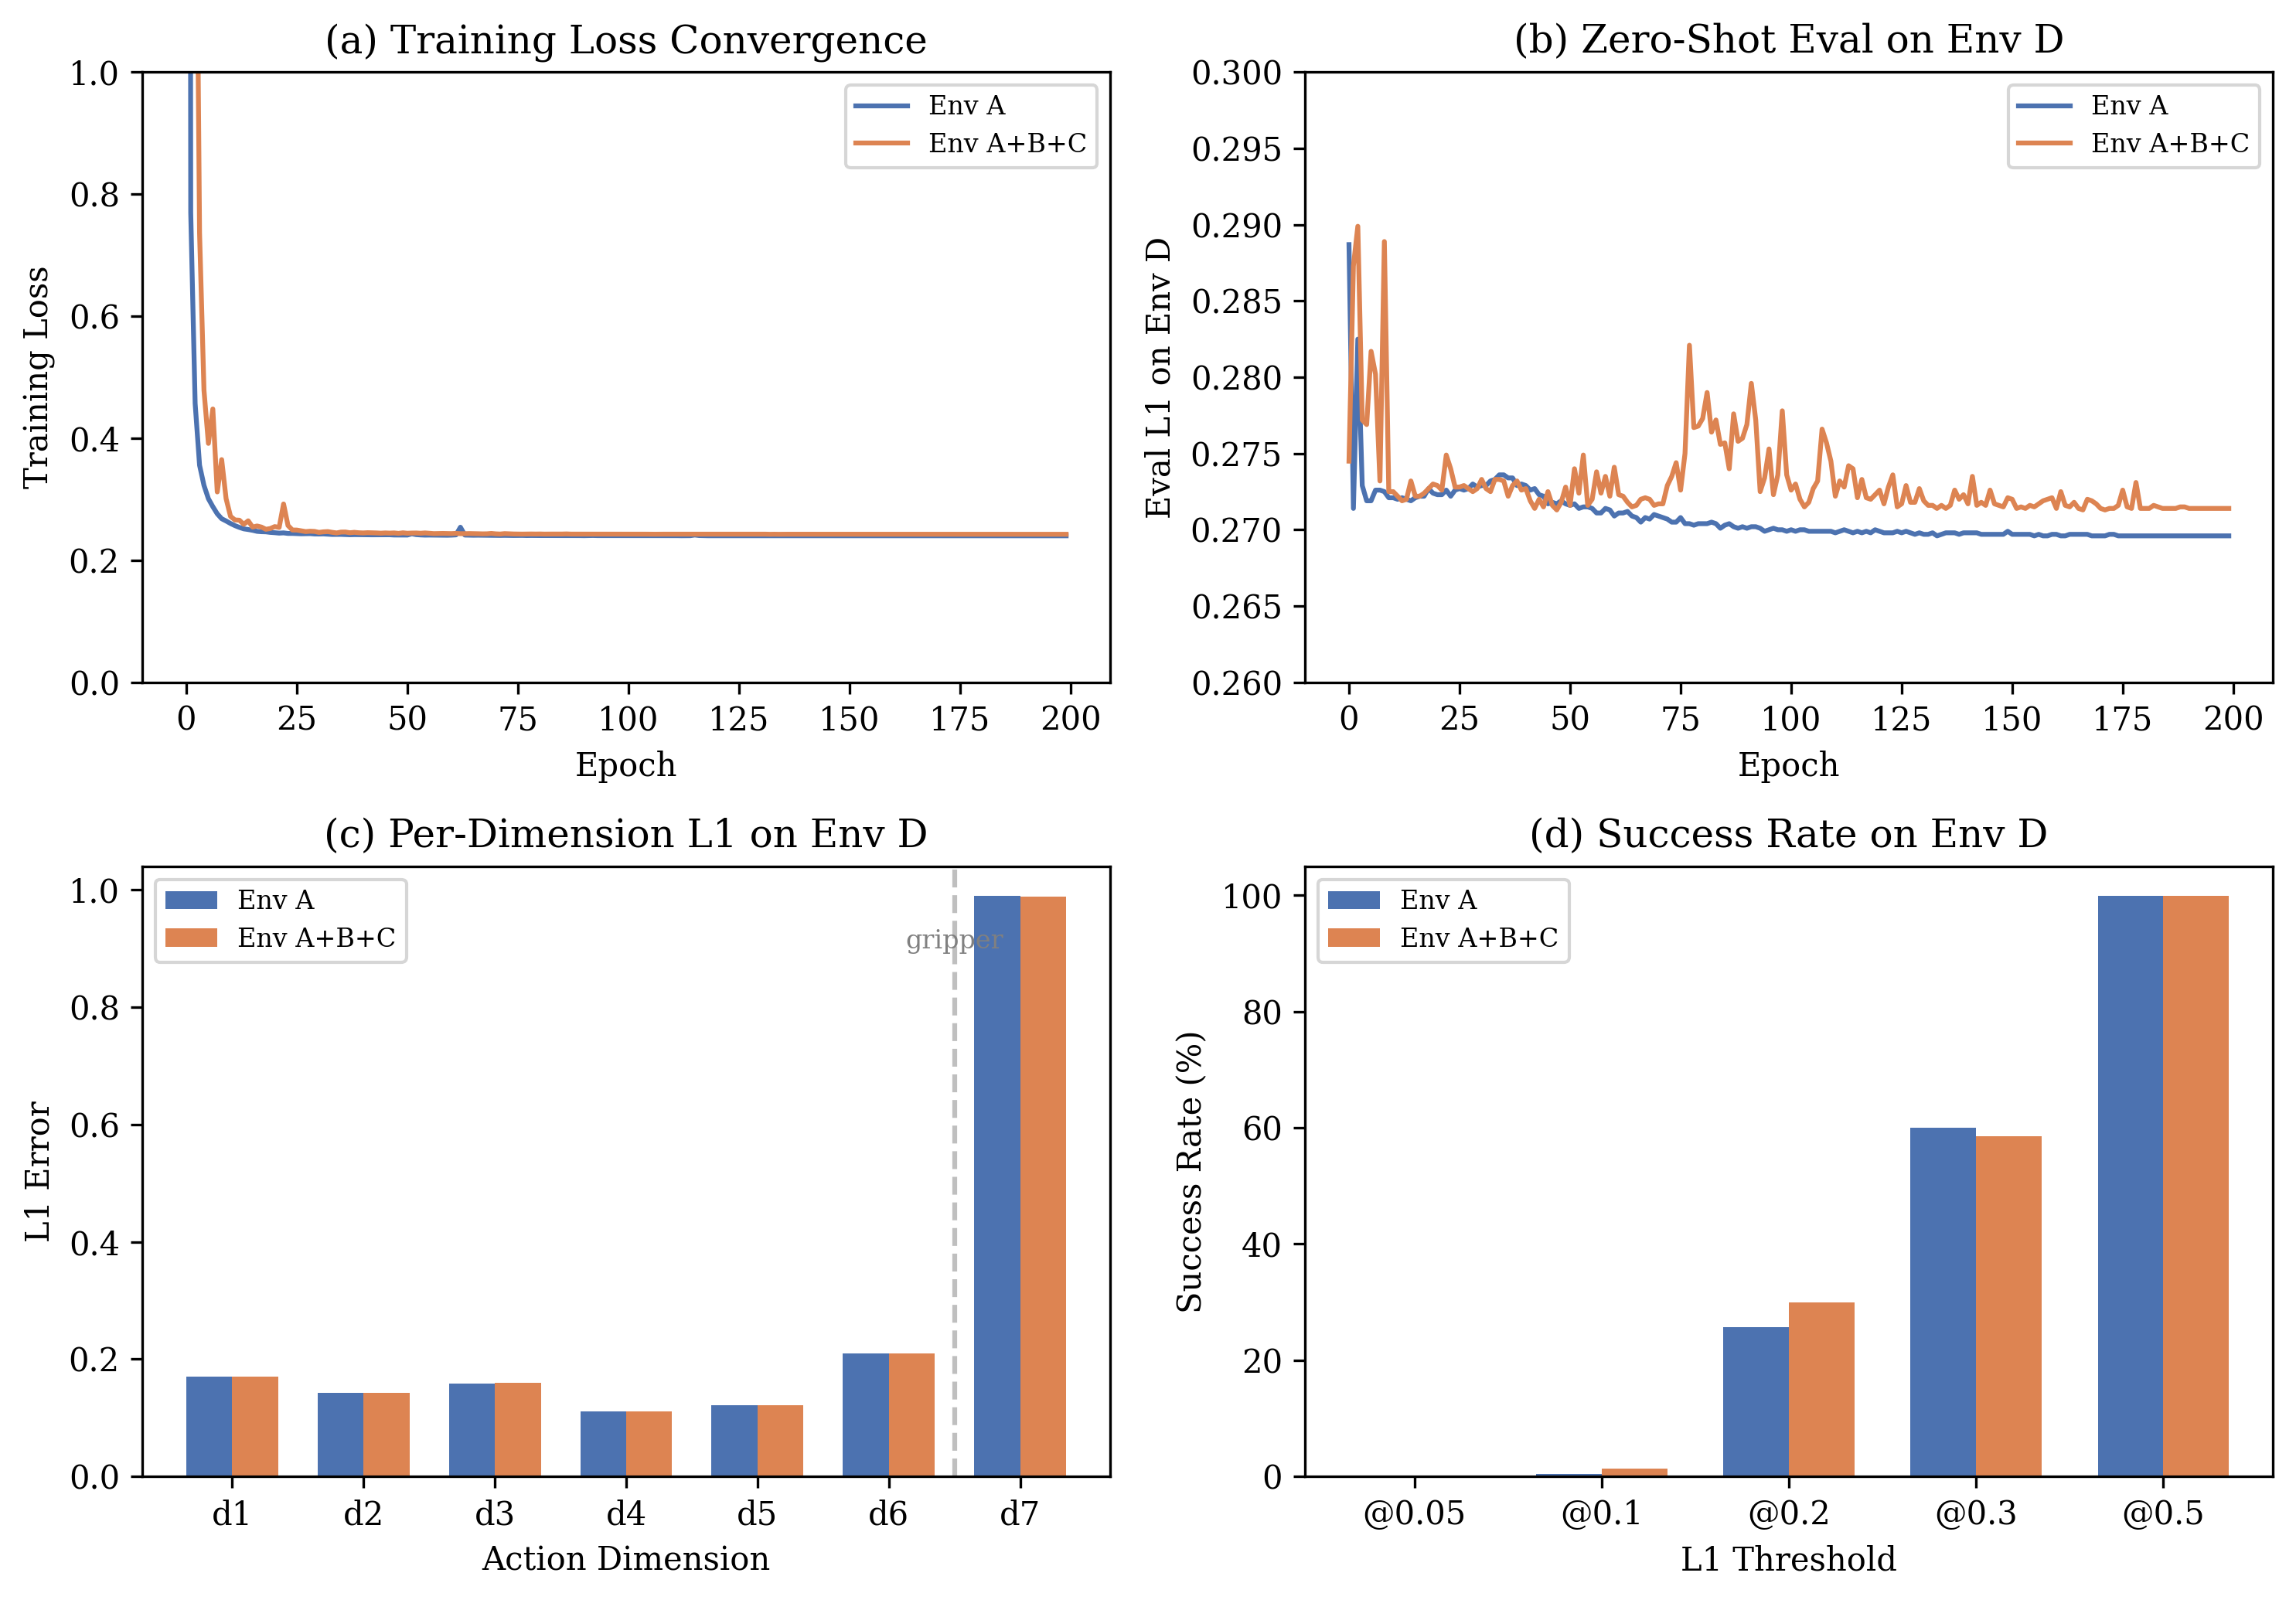
\includegraphics[width=\columnwidth]{figures/act_official_results.png}
\caption{Official LeRobot ACT results. \textbf{(a)} Training loss convergence for Env~A and Env~A+B+C. \textbf{(b)} Zero-shot evaluation L1 on unseen Env~D. \textbf{(c)} Per-dimension L1 error breakdown. \textbf{(d)} Success rate at multiple L1 thresholds.}
\label{fig:act_results}
\end{figure}

\begin{table}[h]
\centering
\caption{Cross-environment generalization: official LeRobot ACT on CALVIN. Eval L1 on~D is from the training-time full-set evaluation; per-dimension breakdown and success rates are computed via post-hoc evaluation on 13{,}879 Env~D samples.}
\label{tab:act_results}
\resizebox{\columnwidth}{!}{%
\begin{tabular}{lccc}
\toprule
Metric & Env A & Env A+B+C & Diff \\
\midrule
Training Loss (final) & 0.2401 & 0.2426 & +0.0025 \\
Eval L1 on D (full set) & 0.2696 & 0.2714 & +0.0018 \\
Joint L1 (dims 1--6) & 0.1524 & 0.1525 & +0.0001 \\
Gripper L1 (dim 7) & 0.9907 & 0.9893 & $-$0.0014 \\
SR@0.1 & 0.4\% & \textbf{1.4\%} & \textbf{+1.0\%} \\
SR@0.2 & 25.7\% & \textbf{30.0\%} & \textbf{+4.3\%} \\
SR@0.3 & 60.0\% & 58.6\% & $-$1.4\% \\
SR@0.5 & 100\% & 99.9\% & $-$0.1\% \\
\bottomrule
\end{tabular}%
}
\end{table}

\paragraph{Convergence} Both models converge rapidly within the first 10 epochs (training loss drops from 8.0 to 0.26) and stabilize for the remaining 190 epochs. The Env~A model achieves slightly lower final training loss (0.2401 vs.\ 0.2426), consistent with its smaller training set.

\paragraph{Zero-shot Generalization to Env D} On the unseen environment~D, the overall L1 errors are nearly identical (0.2696 vs.\ 0.2714 on the full eval set), and the per-dimension breakdown confirms this: joint and gripper L1 differ by at most 0.0014 between the two models. Multi-environment training does \emph{not} improve average prediction accuracy on~D.

However, success-rate analysis at multiple thresholds reveals a nuanced picture: at the practical threshold of 0.2, the Env~A+B+C model achieves \textbf{30.0\%} vs.\ \textbf{25.7\%} for Env~A (+4.3\,pp), and at threshold 0.1 it achieves 1.4\% vs.\ 0.4\% (+1.0\,pp). This indicates that while average errors are comparable, the multi-environment model produces fewer large-error outliers, shifting borderline failures into the success band. At looser thresholds (0.3, 0.5), the two models are indistinguishable.

\subsection{Per-Dimension Analysis}

The 7-DOF action space reveals a strong structural pattern (Table~\ref{tab:act_results}, Figure~\ref{fig:act_results}c):
\begin{itemize}
\item \textbf{Joint dimensions (1--6)}: L1 errors range from 0.111 to 0.210, averaging 0.152. Joint~4 (wrist) is the easiest (0.111) and joint~6 (0.210) the hardest. These continuous dimensions are well-predicted.
\item \textbf{Gripper (dim~7)}: L1 error of 0.99---roughly $6.5\times$ higher than the joint average. The gripper is binary (open/close), and the continuous L1 loss poorly fits this discontinuous action. Since gripper error alone ($\approx$1.0) saturates any threshold below 0.5, \textbf{any sample-level success threshold below 0.5 is effectively gated by gripper prediction quality}, making it the primary bottleneck for fine-grained success.
\end{itemize}

\subsection{Action Chunking Robustness}

We train the \emph{official} LeRobot ACT on environment~A with three chunk sizes (10, 30, 50) for 200 epochs each, using identical hyperparameters (lr $= 10^{-4}$, batch~256, L1~loss). Table~\ref{tab:chunk} reports the results.

\begin{table}[h]
\centering
\caption{Action chunking robustness: official ACT on env~A, evaluated zero-shot on env~D. Train Loss is total (action L1 + KL$\times$10); per-dimension L1 is from post-hoc evaluation.}
\label{tab:chunk}
\resizebox{\columnwidth}{!}{%
\begin{tabular}{cccccc}
\toprule
Chunk & Train Loss & Eval L1 (D) & Joint L1 & Gripper L1 & Samples \\
\midrule
10 & 0.033 & \textbf{0.167} & 0.156 & \textbf{0.243} & 42K \\
30 & 0.240 & 0.270 & \textbf{0.152} & 0.991 & 28K \\
50 & 0.049 & 0.208 & 0.173 & 0.451 & 11K \\
\bottomrule
\end{tabular}%
}
\end{table}

\paragraph{Joint vs.\ Gripper Decoupling} The per-dimension breakdown reveals that the overall L1 is governed almost entirely by the \textbf{gripper dimension}, not the joints:

\begin{itemize}
\item \textbf{Joint L1 (dims 1--6)} is stable at 0.15--0.17 across all chunk sizes. Continuous joint trajectories are smooth and predictable regardless of prediction horizon.
\item \textbf{Gripper L1 (dim 7)} varies dramatically: 0.24 (chunk~10) $\to$ 0.99 (chunk~30) $\to$ 0.45 (chunk~50). The gripper is binary ($\pm$1), and its L1 depends on how often the gripper state \emph{flips} within the prediction window.
\end{itemize}

\paragraph{Mechanism} With chunk~10 (short horizon), the gripper rarely flips within 10 steps, so the model can copy the current gripper state and achieve L1~$\approx$0.24. With chunk~30, the window is long enough that most episodes contain at least one gripper transition; unable to predict \emph{when} the flip occurs, the model outputs $\approx$0 (maximum-entropy guess for $\pm$1 targets), yielding L1~$\approx$1.0. Chunk~50 is intermediate: more flips occur, but the longer window also contains longer stable segments that bias the model toward the dominant state, partially recovering (L1~0.45).

\paragraph{Cross-Environment Implications} Under visual distribution shift (Env~A $\to$ Env~D), chunk~10 achieves the lowest open-loop error (0.167) because it avoids the hardest gripper predictions. However, deploying with chunk~10 means re-querying the policy every 10 steps, which sacrifices temporal smoothness and increases the risk of jerky, uncoordinated motions. Chunk~30 (the official ACT default) offers a balance but suffers from near-maximal gripper uncertainty. The choice of chunk size thus involves a three-way trade-off between joint accuracy, gripper predictability, and deployment smoothness.

\section{Technical Challenges and Solutions}

\subsection{CUDA--GL Interoperability for Fantasia3D} \label{sec:egl}

\begin{sloppypar}
Fantasia3D's \texttt{nvdiff-rasterizer} requires nvdiffrast's \texttt{RasterizeGLContext} with CUDA--OpenGL buffer sharing (\texttt{cudaGraphicsGLRegisterBuffer}). In the headless container, this fails with CUDA error~304 because the EGL vendor configuration only registered Mesa (software renderer), not the NVIDIA EGL driver.

\textbf{Fix:} We create an EGL vendor JSON at \path|/usr/share/glvnd/egl_vendor.d/10_nvidia.json| pointing to \path|libEGL_nvidia.so.0|, forcing EGL to use the NVIDIA driver. This enables CUDA--GL interop and unblocks Fantasia3D's SDF rendering pipeline.
\end{sloppypar}

\subsection{SDS Geometry Collapse and SDF Remedy}

DreamFusion's SDS with SD~v1.5 fails to develop 3D geometry: the density field remains a perfect sphere (elongation~1.00) regardless of blob-prior strength or prompt. We diagnose that the learned density contributes only $+$0.08 on top of the blob prior ($\max$~10.0), meaning the SDS geometry gradient is too weak to overcome the initialization.

\textbf{Fix:} Switching to Fantasia3D (\texttt{implicit-sdf}) with Eikonal regularization produces real geometry (elongation~1.57 for ``a pineapple''). The explicit SDF representation, combined with differentiable mesh rasterization via nvdiffrast, provides stronger geometry gradients than the density-volume formulation.

\subsection{Official 3DGS Extension Compilation}

The official gaussian-splatting code requires two CUDA extensions: \texttt{diff-gaussian-rasterization} and \texttt{simple-knn}. We compile both from source (CUDA~12.1 + PyTorch~2.3.1), add \texttt{\_\_init\_\_.py} to \texttt{simple\_knn} (which exports \texttt{distCUDA2}), and set \texttt{LD\_LIBRARY\_PATH} to include PyTorch's \texttt{libc10.so}. We also patch the dataset reader to accept \texttt{SIMPLE\_RADIAL} camera models (treating them as \texttt{SIMPLE\_PINHOLE}).

\subsection{threestudio Environment Repair}

Building \texttt{tinycudann} (required for threestudio's HashGrid encoding) triggers a numpy~2.x upgrade that cascades through the dependency chain. We repair: numpy~$\to$~1.26.4, \texttt{ml\_dtypes}, transformers~$\to$~4.44.0, \texttt{nerfacc}~$\to$~0.5.2, pytorch-lightning~$\to$~2.0.0, and install missing packages (\texttt{envlight}, \texttt{controlnet\_aux}, \texttt{wandb}).

\subsection{Other Issues}
\begin{itemize}
\item \textbf{COLMAP v3.12 binary format}: String camera model names break old readers. Fixed by using the official COLMAP C++ reader (via gaussian-splatting).
\item \textbf{lerobot data format}: CALVIN v2.1 incompatible with v0.4.4. Custom dataset loader implemented.
\item \textbf{Disk space}: \texttt{/tmp} only 30\,GB; all large files redirected to \texttt{/mnt/workspace/}.
\end{itemize}

\section{Conclusion}

We present a complete multi-source 3D asset generation and scene fusion pipeline with three distinct generation pathways. For \textbf{Object~A} (flower pot), real video $\to$ COLMAP $\to$ \emph{official} 3DGS achieves PSNR~31.94---a dramatic improvement over our initial custom trainer (PSNR~20.05, +11.9\,dB). For \textbf{Object~B} (pineapple), we diagnose DreamFusion's SDS geometry collapse (sphere artifact with SD~v1.5) and remedy it by switching to Fantasia3D's SDF representation, producing a tall pineapple shape (elongation~1.57) with PBR texture. For \textbf{Object~C} (cactus), Zero123 on a clean RGBA input produces a columnar mesh (elongation~2.13) after fragment cleanup. The garden background is trained with official 3DGS to PSNR~29.65 (paper-level quality). Key technical contributions include: (1) fixing CUDA--GL interop in a headless container via NVIDIA EGL vendor registration, enabling Fantasia3D; (2) compiling official 3DGS extensions for both Object~A and the garden; (3) diagnosing and documenting the SDS geometry collapse limitation.

For Task~2 (ACT), we train the official LeRobot ACT policy on environment~A and the joint A+B+C split. Both models converge rapidly ($\sim$10 epochs) and achieve nearly identical zero-shot action L1 on the unseen environment~D (0.270 vs.\ 0.271). Per-dimension analysis reveals that the binary gripper dimension (L1~$\approx$0.99) dominates the error, roughly $6.5\times$ the joint-average L1 (0.15). Multi-environment training yields a modest but consistent improvement in success rate at the practical L1 threshold of 0.2 (30.0\% vs.\ 25.7\%, +4.3\,pp), indicating fewer large-error outliers rather than better average prediction. Action chunking analysis shows that chunk size primarily affects gripper predictability: short chunks (10) keep gripper L1 at 0.24 because state flips are rare within the window, while the default chunk~30 suffers near-maximal uncertainty (L1~0.99).

\bibliographystyle{plain}
\begin{thebibliography}{10}

\bibitem{kerbl2023gaussian}
Bernhard Kerbl, Georgios Kopanas, Thomas Leimk{\"u}hler, and George Drettakis.
\newblock 3d gaussian splatting for real-time radiance field rendering.
\newblock \emph{ACM Transactions on Graphics}, 42(4), 2023.

\bibitem{ye2024gsplat}
Viktor Ye, Jinglin Liang, Yihua Cheng, and Yiwen Xu.
\newblock gsplat: An open-source library for gaussian splatting.
\newblock \emph{arXiv preprint arXiv:2407.05432}, 2024.

\bibitem{lin2023magic3d}
Chen-Hsuan Lin, Jun Gao, Luming Tang, Towaki Takikawa, Xiaohui Zeng, Xun Huang, Karsten Kreis, Sanja Fidler, James Fung, and Tsung-Yi Lin.
\newblock Magic3d: High-resolution text-to-3d content creation.
\newblock \emph{ICLR}, 2023.

\bibitem{poole2022dreamfusion}
Ben Poole, Ajay Jain, Jonathan T. Barron, and Ben Mildenhall.
\newblock Dreamfusion: Text-to-3d using 2d diffusion.
\newblock \emph{arXiv preprint arXiv:2209.14988}, 2022.

\bibitem{chen2023fantasia3d}
Rui Chen, Yongwei Chen, Ningxin Jiao, and Kui Jia.
\newblock Fantasia3d: Disentangling geometry and appearance for high-quality text-to-3d content creation.
\newblock \emph{ICCV}, 2023.

\bibitem{liu2023zero123}
Ruoxi Liu, Rundi Wu, Weijian Luo, Hao Tan, Xingyu Chen, Zhiwen Lyu, and Yuwei Guo.
\newblock Zero-1-to-3: Zero-shot one image to 3d object generation.
\newblock \emph{ICCV}, 2023.

\bibitem{threestudio}
threestudio team.
\newblock threestudio: An open-source framework for 3d generation.
\newblock \url{https://github.com/threestudio/threestudio}, 2023.

\bibitem{zhao2023act}
Tony Z. Zhao, Vikash Kumar, Chelsea Finn, and Sergey Levine.
\newblock Learning fine-grained bimanual manipulation using low-cost hardware.
\newblock \emph{RSS}, 2023.

\bibitem{mees2022calvin}
Oleh Mees, Lukas Hermann, Emre Ugur, and Wolfram Burgard.
\newblock Calvin: A benchmark for language-conditioned policy learning for long-horizon robot manipulation tasks.
\newblock \emph{RSS}, 2022.

\bibitem{lorensen1987marching}
William E. Lorensen and Harvey E. Cline.
\newblock Marching cubes: A high resolution 3d surface construction algorithm.
\newblock \emph{SIGGRAPH}, 1987.

\bibitem{barron2022mipnerf360}
Jonathan T. Barron, Ben Mildenhall, Dor Verbin, Pratul P. Srinivasan, and Peter Hedman.
\newblock Mip-nerf 360: Unbounded anti-aliased geometric radiance fields.
\newblock \emph{CVPR}, 2022.

\end{thebibliography}

\appendix

\section{Experimental Setup Details}

\subsection{Hardware}
8$\times$ NVIDIA A100-80GB GPUs, PyTorch~2.4.1+cu121, CUDA~12.1, Python~3.11.

\subsection{Key Configuration Parameters}

\begin{table}[h]
\centering
\caption{Training configuration for all experiments.}
\resizebox{\columnwidth}{!}{%
\begin{tabular}{lll}
\toprule
Parameter & 3DGS (Object~A + Garden) & Official LeRobot ACT \\
\midrule
Iterations/Epochs & 30{,}000 & 200 \\
Learning rate & Adaptive (exp.\ decay) & $1 \times 10^{-4}$ \\
Optimizer & Adam (official) & AdamW (wd $= 10^{-4}$) \\
Batch size & N/A (full image) & 1{,}536 (A) / 12{,}288 (ABC) \\
LR schedule & Exponential decay & Cosine annealing \\
Gradient clip & --- & 1.0 \\
Loss & Photometric $L_1$ + D-SSIM & $L_1$ action + KL $\times$ 10 \\
Architecture & 3DGS (SH deg~3) & ResNet-18 + 4L Trans. \\
Parameters & 976K Gaussians & 51{,,}571{,}591 \\
GPUs & 1$\times$A100 & 6$\times$A100 (DataParallel) \\
\bottomrule
\end{tabular}%
}
\end{table}

\section*{Resources}

\begin{itemize}
\item \textbf{GitHub Repository}: \url{https://github.com/ZhenYongWei/sp-hw3}
\item \textbf{Model Weights}: Included in the repository under \texttt{checkpoints/} (via Git LFS)
\end{itemize}

\end{document}
